% arara: pdflatex: {files: [../MathSACpr2014]}
% !arara: indent: {overwrite: yes}
\chapter{Pathways diagram}\label{app:sec:pathways}

\begin{figure}[!htb]
  \centering
  % arara: pdflatex
% !arara: indent: {overwrite: yes}
\documentclass[tikz]{standalone}

\usepackage{tikz}
\usetikzlibrary{positioning}

\begin{document}
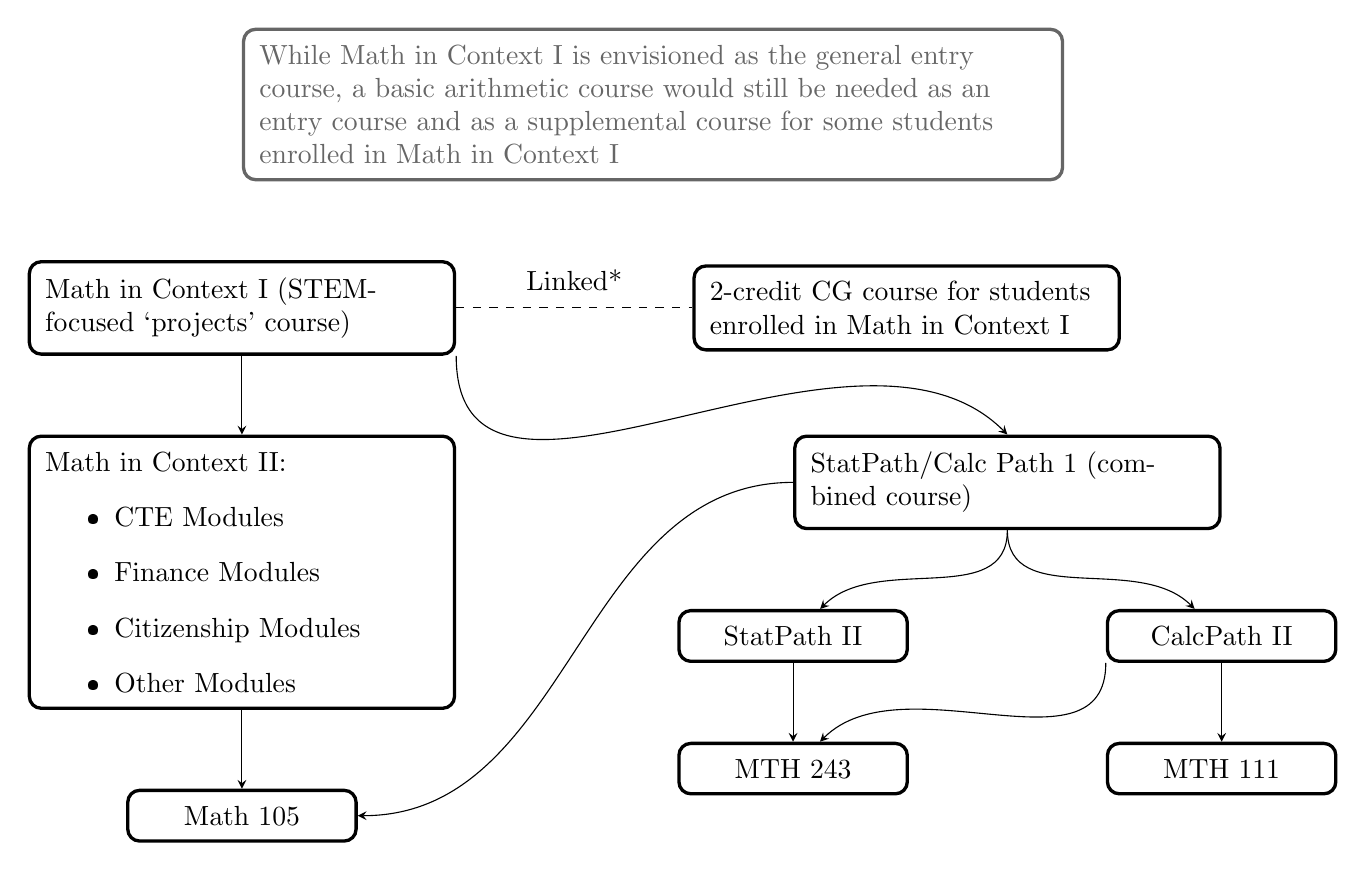
\begin{tikzpicture}[
		>=stealth,
		every node/.append style={
			draw=black,
			rounded corners=1ex,
			very thick,
			inner sep=.2cm,
		},
		wide/.style={text width=5cm},
		narrow/.style={text width=2.5cm,align=center},
	]
	\node[text width=10cm,black!60] (entrycourse) at (0,0) {While Math in Context I is envisioned as the general
		entry course, a basic arithmetic course would still be needed as an entry course
	and as a supplemental course for some students enrolled in Math in Context I};
	% left side of the picture
	\node[wide] (context1) [below=of entrycourse.south west]{Math in Context
	I (STEM-focused `projects' course)};
	\node[wide] (cgcourse) [right =3cm of context1]{2-credit CG course for students enrolled in Math in Context I};
	\node[wide](context2) [below=of context1]{
		Math in Context II:
		\begin{itemize}
			\item CTE Modules
			\item Finance Modules
			\item Citizenship Modules
			\item Other Modules
		\end{itemize}
	};
	\node[narrow] (math105) [below=of context2]{Math 105};
	% right side of the picture
	\node[wide] (combined) [xshift=7cm,below=of context1.south east] {StatPath/Calc Path 1 (combined course)};
	\node[narrow] (stat2) [below=of combined.south west] {StatPath II};
	\node[narrow] (calc2) [below=of combined.south east] {CalcPath II};
	\node[narrow] (math243) [below=of stat2] {MTH 243};
	\node[narrow] (math111) [below=of calc2] {MTH 111};
	% draw the connection lines
	\draw[dashed] (context1)--(cgcourse) node [draw=none,pos=0.5,anchor=south]{Linked*};
	\draw[->] (context1.south east) to[out=270,in=135] (combined.north);
	\draw[->] (context1) -- (context2);
	\draw[->] (context2) -- (math105);
	\draw[->] (combined) to[out=270,in=45] (stat2);
	\draw[->] (combined) to[out=270,in=135] (calc2);
	\draw[->] (combined.west) to[out=180,in=0] (math105.east);
	\draw[->] (stat2) -- (math243);
	\draw[->] (calc2) -- (math111);
	\draw[->] (calc2.south west) to[out=270,in=45] (math243);
\end{tikzpicture}
\end{document}

  \caption{PCC MathPaths-- Draft Version III (01/17/2014)}
\end{figure}

*Every student in a given section of Math in Context I 
would also be enrolled in a common section of the CG 
course.  The instructors of a given pair of courses 
would work in a collaborative fashion and ideally visit 
one another's classes, especially the first week. 

Unlinked sections of the CG course would be offered 
for entry level DE mathematics students whose initial 
placement is `above' Math in Context I.  Students who 
pass Math in Context I but not the attendant CG course 
might be required to retake the course. 

